% ---------------------------------------------------------------------------
% CHAPTER 4 (RQ1). Rewritten on 2026-11-16 with AI assistance (Claude) from
% the reviewed drafts of 2026-11-15 (docs/thesis/reviews/2026-11-15-g-raw/
% results.json, part ch4: rewrites R1 to R6, drafts "Answer to RQ1", "Parse
% once, fail visibly" and "Planning the Deck Without a Model"), their
% verification (verify.json) and the author's decisions of 16 November.
% New: Section 4.2 "How the Pipeline Developed" (label sec:c4-lineage), written
% only from commits, PR texts, commit messages and code at the pin; the
% re-run counts of the Pipeline History Workbench are not cited, because their
% scripts are not in the repository. The lineage table stays in the appendix
% (tab:lineage). No worked example, so the pipeline diagram (fig:pipeline)
% stays in the appendix. Code facts re-checked at the pin \thesisCommit.
% Every passage that left the chapter is kept verbatim in the defence notes
% (Chapter 4, 16 November).
% Labels kept: ch:content, sec:c4-requirements, fig:page-types, sec:pipeline,
% sec:async, sec:idempotency, sec:c4-deck-plan, sec:routing,
% sec:c4-evaluation, sec:c4-routing-study, fig:routing, sec:parser-bench,
% fig:parser-bench, sec:c4-answer. Moved: sec:c4-lineage, now on its own
% section.
% The author must read, revise and own every sentence before submission.
% ---------------------------------------------------------------------------
\chapter{From PDF to Structured Pages}
\label{ch:content}

This chapter answers RQ1. It describes the input, how the pipeline developed,
and the pipeline at the pin, and then two evaluations: a routing study on
1{,}593 pages and a pre-registered blind benchmark of eleven text extraction
methods.

\section{The Input and What It Demands}
\label{sec:c4-requirements}

The input is a deck, the slides of one lecture exported as one PDF. Inside the
system it becomes a Lesson, and each of its pages a page
(\cref{tab:vocabulary}).

The prototype was built for the Database Systems course at the University of
Marburg, and its eleven decks, ten in English and one German introduction,
are part of the corpus. To see whether the pipeline also works on other
slides, we added fourteen German decks of a second Marburg course, System
Software and Computer Communication (\emph{Systemsoftware und
Rechnerkommunikation}). Together they form the corpus of this
chapter: 25 decks with 1{,}593 pages. The benchmark adds one
software-engineering deck and two exercise sheets. All are
born-digital. Pages from both
courses were used to calibrate the routing rule, so the second course is not
an independent test of it (\cref{sec:c4-routing-study}).

The input makes three demands on the design.

\begin{description}
  \item[Pages differ in kind.] This is what \emph{heterogeneous} means here:
    no single way of reading fits every page. A born-digital PDF stores its
    words in its text layer and its pictures as embedded images. A deck mixes dense text, bullet lists with
    formulas, diagrams drawn with lines, and pictures (\cref{fig:page-types}).
    In the text layer a drawn diagram is only a handful of loose labels, and
    lines that repeat on most pages, such as the footer and page number of
    the systems decks or the course name of the database decks, look like any
    other content. And 421 of the 1{,}593 pages hold at least one
    \emph{figure}, an embedded image that is neither a logo nor the page
    background.
  \item[A learner should not wait.] The learner should start on a deck at once,
    as with any PDF, while the system prepares everything else in the
    background. Preparing a deck can take minutes: in one measured run of
    October 2026, an 82-page deck took about twelve minutes from upload to a
    complete reading view
    (\code{docs/\allowbreak thesis/\allowbreak evidence/\allowbreak reader-timing.md}).
    The pipeline therefore runs behind the learner's reading, not in front of it.
  \item[Model calls cost money and fail.] The free tiers of hosted models
    stopped bulk parsing within minutes, because they limit the calls they
    accept per minute or per day (commit \code{a12666cd}). A self-hosted model on a
    university GPU server would have needed time and experience that we did
    not have, and its cost would have been harder to compare, so we chose a
    paid API. With a provider that charges per token, every call has a price,
    which makes the number of model calls per deck a design variable. It also
    frames the central comparison of this chapter: whether a page is best read
    by a text extractor, by a vision model, or by both.
\end{description}

\begin{figure}[htbp]
  \centering
  {\footnotesize\setlength{\tabcolsep}{3pt}%
  \begin{tabular}{@{}p{0.235\textwidth}p{0.235\textwidth}p{0.235\textwidth}p{0.235\textwidth}@{}}
    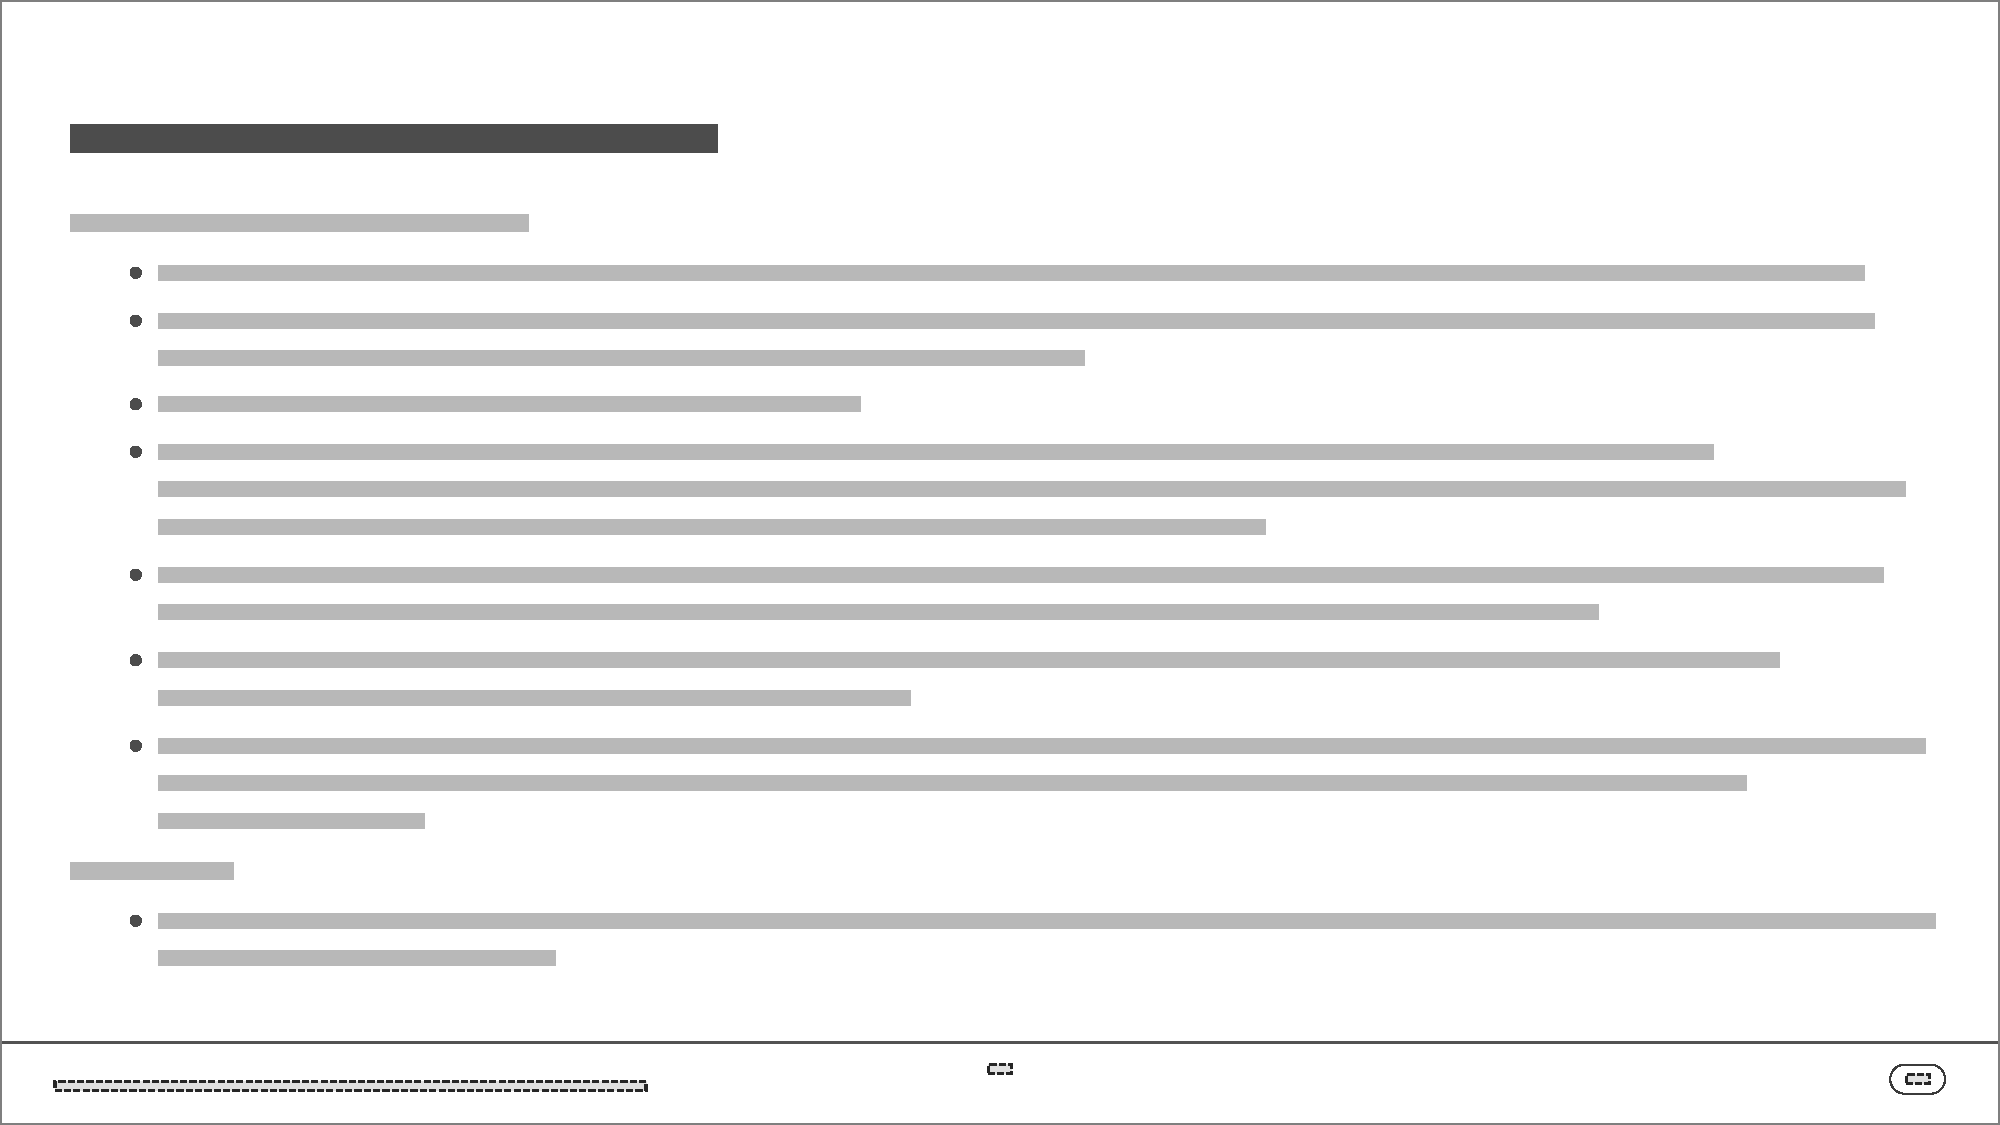
\includegraphics[width=0.235\textwidth]{f26-page-types-a} &
    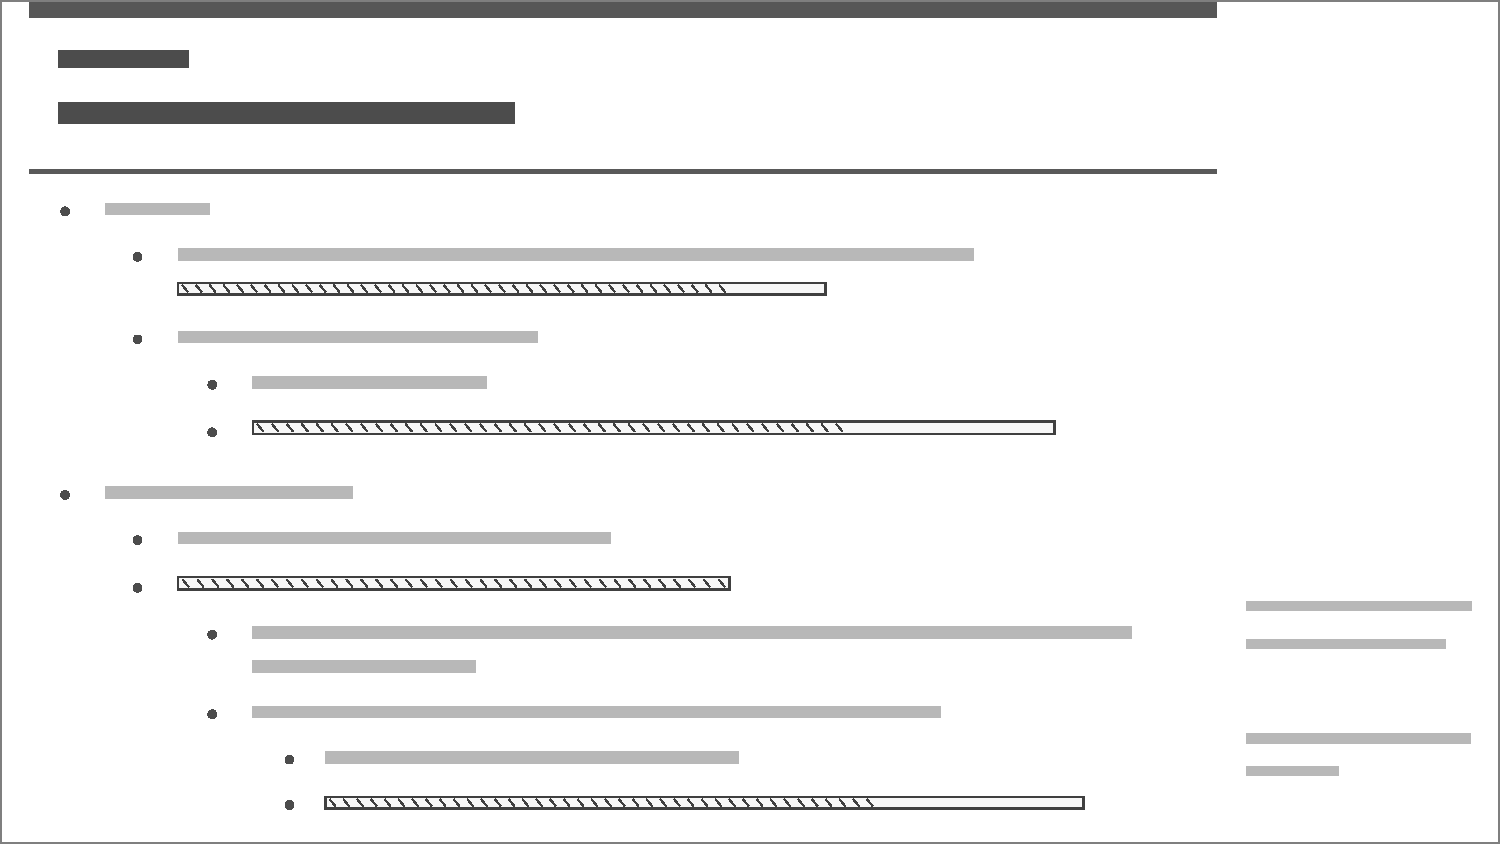
\includegraphics[width=0.235\textwidth]{f26-page-types-b} &
    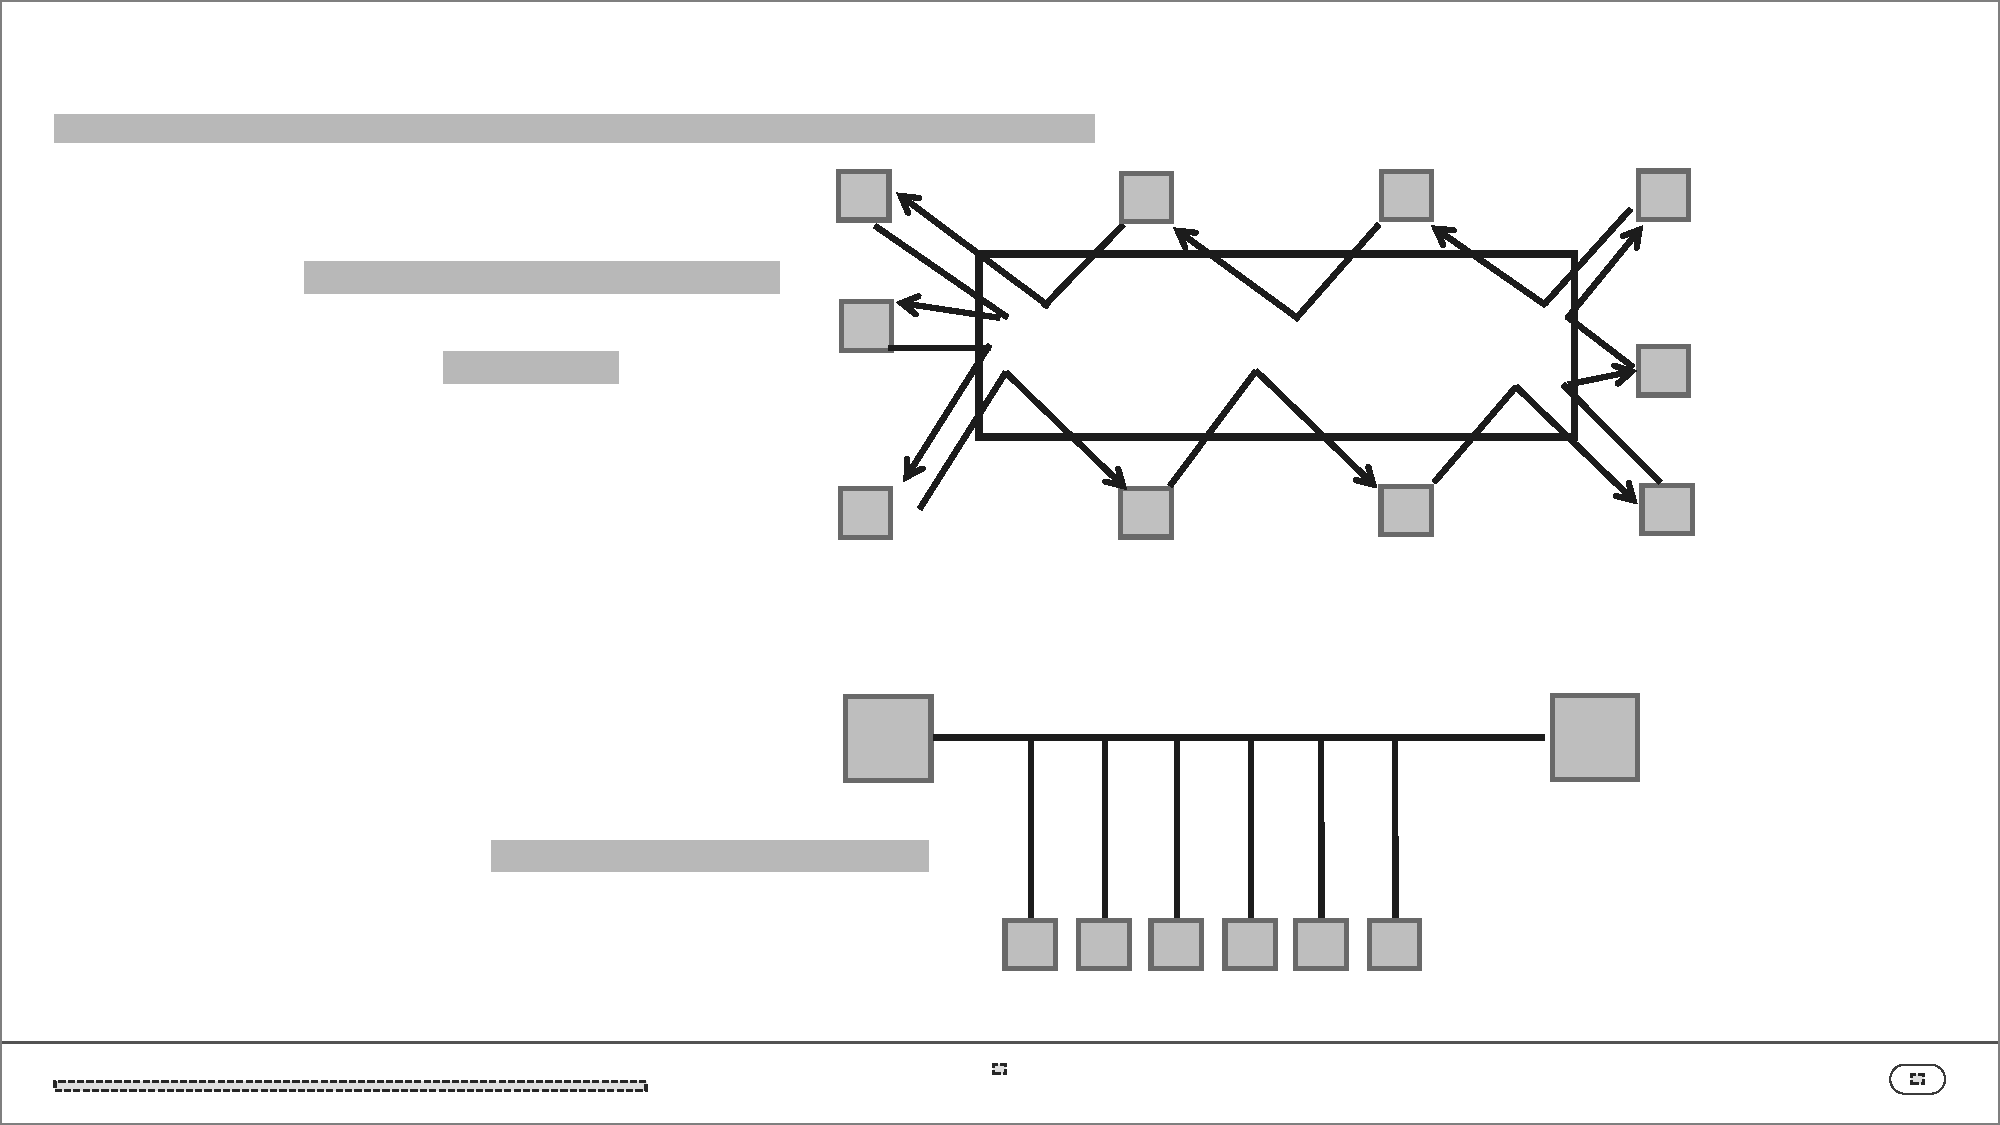
\includegraphics[width=0.235\textwidth]{f26-page-types-c} &
    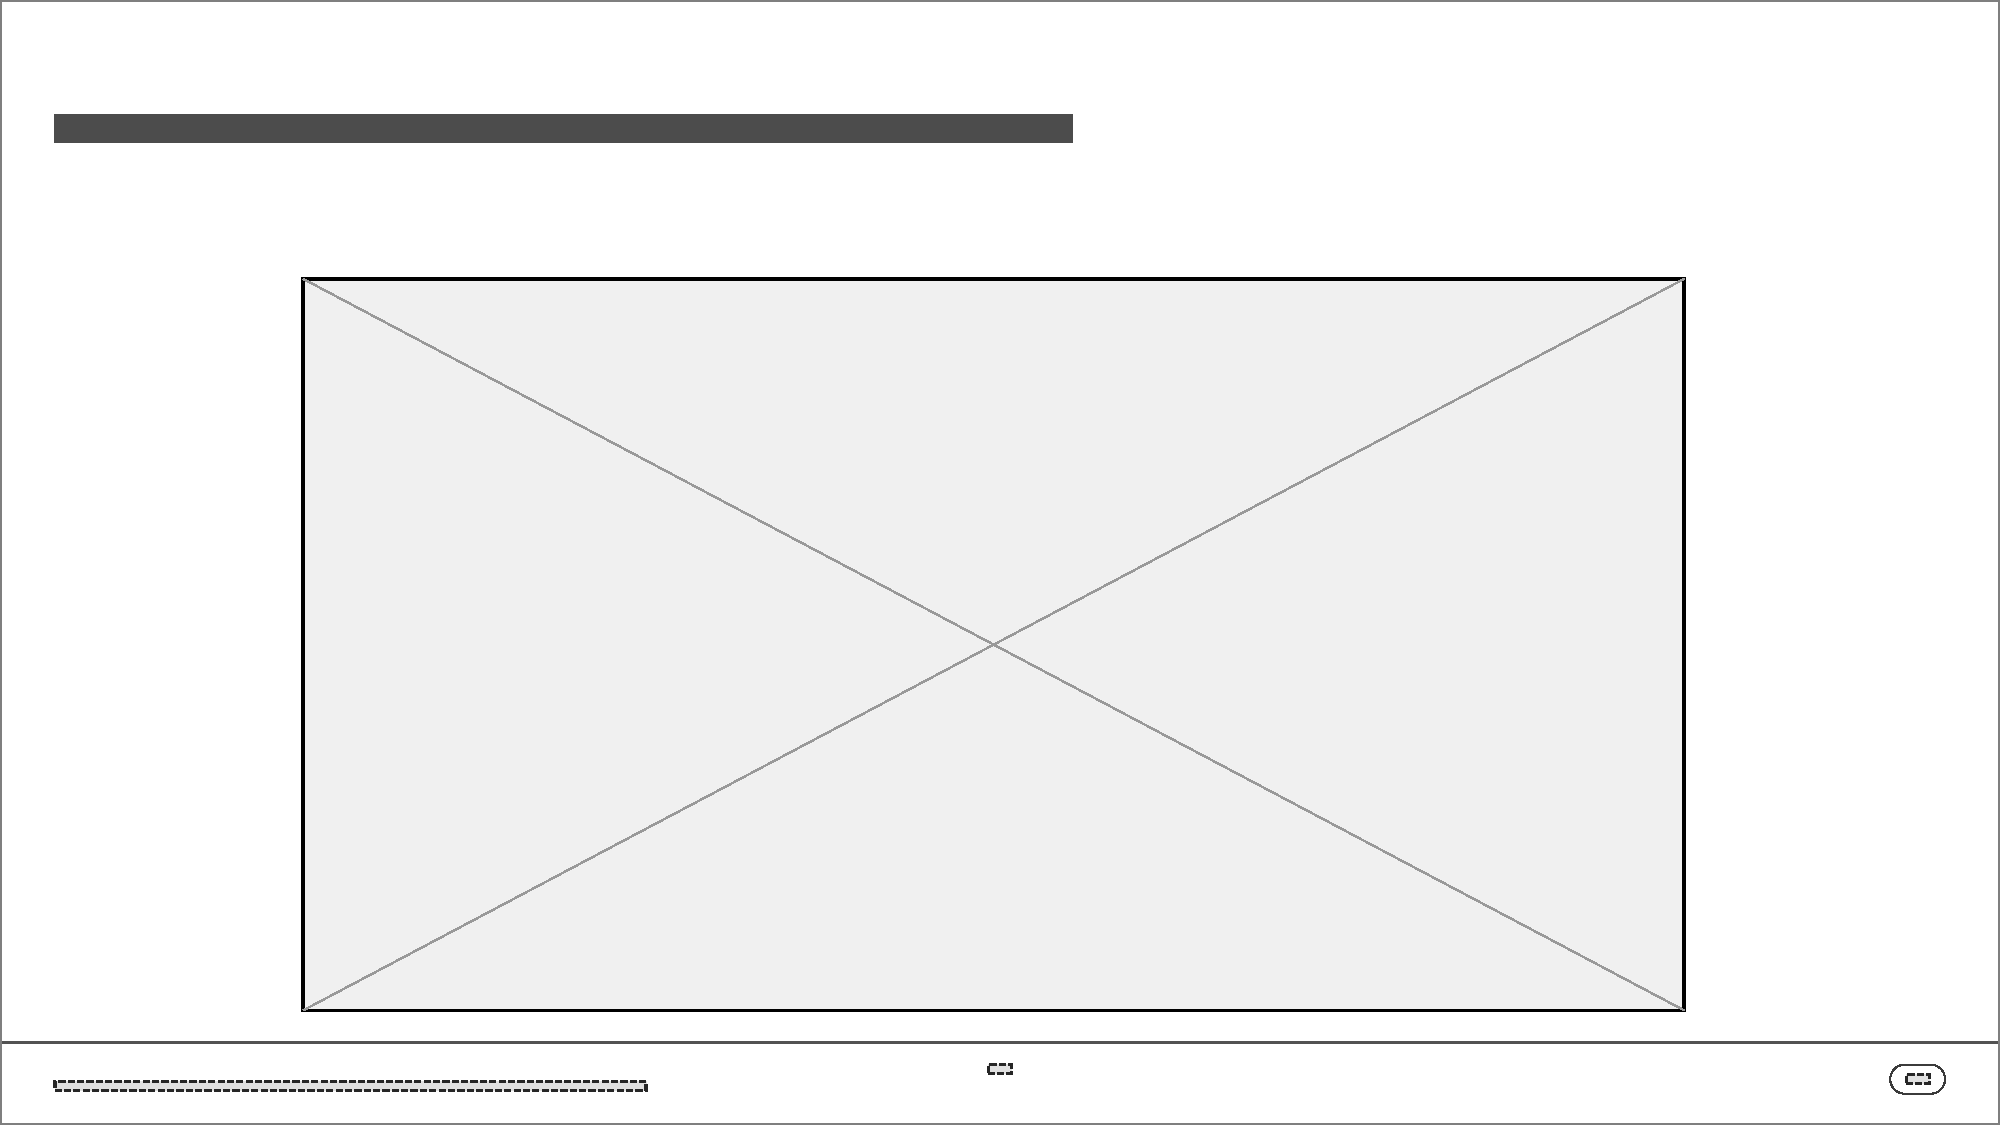
\includegraphics[width=0.235\textwidth]{f26-page-types-d} \tabularnewline
    \raggedright (a) Dense text: 1{,}345 characters; text. &
    \raggedright (b) Bullets and formulas: 641 characters; text. &
    \raggedright (c) Drawn diagram: 63 characters of labels; text. &
    \raggedright (d) Plot: 32 characters, image on 45\,\% of the page; vision.
    \tabularnewline
  \end{tabular}\par}
  \caption{Four pages of the corpus, drawn from their real layout: each line
    of text is a bar, bullets are dots, lines with formula symbols are
    hatched, a footer is dashed, and an embedded image is a crossed box; the
    content of the slides is not shown. Character counts leave footers out;
    page~(d) has 97 with its footer. Each label ends with how the routing rule
    of \cref{sec:routing} reads the page. Script:
    \code{docs/\allowbreak thesis/\allowbreak experiments/\allowbreak page-types/}.}
  \label{fig:page-types}
\end{figure}

These three demands are the yardstick for the rest of the chapter: how the
pipeline handles a page whose meaning lies in a figure, how soon a learner can
read, and what a deck costs.

\section{How the Pipeline Developed}
\label{sec:c4-lineage}

The pipeline went through five versions in 2026, v1 to v5;
\cref{tab:lineage} in \cref{app:detail} lists them by month, with the filter of
v1 and three later rebuilds of v5 as rows of their own. Before any of them, a
lecturer typed each slide into a form with a title, the content, a summary,
and one question (\code{184e5742}). Every version since has filled these
fields from a PDF, although at the pin the questions come as one quiz per
deck.

\paragraph{v1, February to April: a model on every page.}
The first parser read each page's text with pypdf, a Python library for PDF
files, and, as our supervisor had suggested, buttons in the lecturer's form let
a model write a page's summary or question on demand (\code{be25cc1d}). In the
same month a model began to write a rewrite, a summary, and a question for
every page at upload, in three calls per page and from March in four, the
fourth for a title (\code{4c23d254}, \code{10296bef}). In March the co-developer added a filter that kept pages
without teaching content, such as title pages, from the model, because they
wasted tokens and produced useless questions; it judged a page by its text
alone (\code{bfbe6c09}). At the end of March the co-developer also merged the
four calls into one (\code{76aa4b42}). In April
the extractor changed to PyMuPDF (\cref{sec:stack}), and every page went to a
vision model when one was available (PR~\#4).

\paragraph{v2, May to June: look at the page first.}
v2 measured each page before any model call and sent it by fixed rules to a
text, vision, or table route, or skipped it (\code{7ffb0cd2}). But its second
rule skipped every page that the filter of v1 had marked as not teaching, so
the old filter still decided first (\code{a801c31f}).

\paragraph{v3, May to July: built beside v2.}
v3 moved parsing into a job queue, Arq~\cite{arq}, on Redis
(\code{6ce7b5f1}). Its five stages record each parse, a \emph{run}, and
each page's progress in the database, so that a run can resume after a crash
(\code{parser/\allowbreak orchestrator.py} at \code{6ce7b5f1}). v3 never served an upload: its extractor,
Docling~\cite{auer2024docling}, would have made every build of the production
image more than half an hour longer, so the image left Docling out and ran v2
(\code{requirements-docker.txt} at \code{6ce7b5f1}).

\paragraph{v4, May to June: a voice without sight.}
v4, a port of an earlier Node.js version, asked the model to explain each page
as a professor would in one continuous lecture (\code{6ce7b5f1}). It had no
router: an offline check in June sent 142 of the 143 pages of a
machine-learning lecture exported from PowerPoint to text (message of commit
\code{4f19bd1e}).

\paragraph{v5, since June: one path, written by the server.}
We built v5 in one day in June on the job queue and run table of v3. It fixed
the two things that v4 could not do: the server writes every Lesson, page, and
question to the database itself, where before the browser had saved them, and
a page can go to a model that sees its image (\code{4f19bd1e}). By the end of
that day one call per page wrote each page, because one failed call for a
group had left eight pages blank, and a page with fewer than 25 characters of
text went to vision (\code{bd03f1d5}). With this rewrite the filter of v1 left
the path, because the new code no longer called it. Since July v5 has been the
only path (\code{a65b0f9d}). It sends text pages in groups again, because one
call per page made its most expensive step about eight times as costly, and a
failed group falls back to one call per page (\code{49994d51}).

\paragraph{What the versions left.}
The pipeline of \cref{sec:pipeline} keeps from v1 the fields of a page and the
original page shown with the generated text, from v2 the decision per page
before any model call, from v3 the job queue and run table, from v4 the calls
that write a deck's title and quiz, and from v5 the server that writes each
page (\code{4c23d254}, \code{a65b0f9d}).

\section{The Pipeline as Built}
\label{sec:pipeline}

One pipeline is in use: v5, kept in
\code{backend/\allowbreak services/\allowbreak parser/\allowbreak unified\_orchestrator.py}.
\Cref{fig:pipeline} in \cref{app:detail} draws its path from an upload to a
readable page in the terms of the code.

\paragraph{What we mean by reliable.} We call the pipeline reliable if it
keeps two promises: every upload that the API accepts ends either as a
readable Lesson or as a failure that the learner sees, and the same file is
not parsed twice for one uploader. The API refuses an upload that breaks a
limit before it queues a job: more than 50\,MB or 300 pages, more uploads than
a student's monthly quota (five by default, 30 in production), or a queue that
already holds 50 jobs
(\code{core/\allowbreak config.py:90,101,134}, \code{upload\_service.py:13}).
Tests at the pin check each mechanism, among them a full run against a real
database (\code{test\_unified\_pipeline\_e2e.py}). In production, pipeline v5
ran 115 parses between June and November 2026, our own uploads included: 99
completed, 16 failed, and none was left unfinished
(\code{docs/\allowbreak thesis/\allowbreak evidence/\allowbreak parse-runs.md}).
These counts show that failures surfaced as failures; they are too few, and
the load too light, to measure reliability under real use.

\subsection{Asynchronous Processing, Page by Page}
\label{sec:async}

The API hands each parse to a durable queue and returns, and a worker takes
the job. A job that runs longer than 900~seconds is cancelled, and its run
ends as failed with a message to the user (\code{arq\_worker.py:52--56,362}). In
November 2026 this happened to two decks of 78 and 104 pages, although decks
of 82 to 136 pages had finished in October, so the page count alone does not
predict it. We did not measure where the limit lies.

Inside one job the pipeline works in a fixed order. It extracts the text of
every page with PyMuPDF and plans the deck without a model
(\cref{sec:c4-deck-plan}). A model then writes the Lesson's title and summary
and, for every page, a title and a short summary; we call this step
\emph{synthesis}. A page keeps its own text unless it has none; then the
vision model writes it (\code{unified\_orchestrator.py:1159--1165}). Text pages
go to the model in groups of up to eight per call, and a page that needs its
image goes to a vision model alone (\cref{sec:routing}). We tried 12, then
5, then 8 pages per call in May 2026 and kept 8, which worked on our decks; we
did not measure other values. The job then writes the deck quiz
(\cref{ch:trust}) and a \emph{parse receipt}, a record of how each page was
read and of each text-model call with its tokens and cost; vision and
embedding calls are not metered (\code{unified\_orchestrator.py:546--547}). It
translates the Lesson and its quiz into the other of English and German and
waits for the \emph{embeddings}, lists of numbers that place texts with
similar meaning close together, with which the ask bar finds pages for a
question.

The job creates the Lesson before it writes the first page and stores each
page as soon as it is ready. Meanwhile the reading view on the uploader's
device opens the uploaded PDF itself, so the learner reads the original pages
at once and sees each generated page as soon as it exists
(\code{useEarlyReading.ts}).

\paragraph{Parse once, fail visibly.}
\label{sec:idempotency}
The SHA-256 hash of a file, a fingerprint computed from its bytes, is its
identity. A unique key on hash, pipeline version, and uploader, a lock on the
hash while the worker parses, and the replay of a finished run keep one
uploader's file from being parsed twice unless a re-parse is forced, as long
as Redis, which holds the lock, is reachable
(\code{unified\_orchestrator.py:793--877}). A parse is not shared between
uploaders, because the embeddings are attached to a Lesson through the file's
hash, and a shared parse would silently move them to whichever uploader parsed
last (\code{unified\_orchestrator.py:785--791}). Two students who upload the
same deck therefore pay for two parses. A failed job keeps the pages it has
written and marks its run as failed, and the user can retry. A sweep every ten
minutes closes stuck runs and fails a run that has waited in the queue for six
hours (\code{arq\_worker.py:67,72}). The run of a second uploader whose
identical file arrives while the first parse runs ends this way: its job finds
the lock held and leaves the run queued
(\code{unified\_orchestrator.py:871--877}).

\subsection{Planning the Deck Without a Model}
\label{sec:c4-deck-plan}

A deterministic step plans the deck before any model call: the same pages
always give the same plan (\code{deck\_plan.py:1--13}). The plan does three
things. It finds the deck's \emph{boilerplate}, lines that recur on at least
60\,\% of its pages, such as a course name in the header, and hides them from
the model, while the stored page keeps them; a line of real content that
recurs as often is hidden too. It gives each page one of eight roles, such as
title, agenda, section start, or summary, by simple rules, most of them on its
first line.
And it groups the pages into sections and picks, spread over all sections, up
to ten pages for the deck quiz and up to fifteen for the Lesson's title and
summary (\code{synthesis.py:176}, \code{deck\_plan.py:250--259}). We chose the
60\,\% without measuring it; at 50 or 70\,\%, the boilerplate of three or four
of the 25 decks changes
(\code{docs/\allowbreak thesis/\allowbreak experiments/\allowbreak deck-plan-threshold/}).
Because the step calls no model, we could test it thoroughly, also with
property-based tests, which check a rule on many generated decks.

Before the plan, which arrived in October 2026, the title step read the first
15 pages of a deck and the quiz step the first ten
(\code{deck\_plan.py:3--4}). The quiz step kept only pages with more than 50
characters and numbered them from one, as Slide~1 to Slide~10, so a question
could cite the wrong page; in
production, all 524 deck-quiz questions written before the plan sat on the
first eleven pages of their decks, and since the plan they reach page 121
(\code{docs/\allowbreak thesis/\allowbreak evidence/\allowbreak deck-quiz-anchors.md}).
This counts where the questions point, not whether they are good.

\subsection{Routing: Text versus Vision}
\label{sec:routing}

One function decides how each page is read
(\code{page\_blocks.py:213--219}). It looks at the PDF page itself, so the
decision does not depend on which extractor supplied the text. It measures
two things: how many characters of text the page has, and how much of the
page its figures cover. Running footers, text blocks that start in the bottom
tenth of the page in smaller type than its body text, such as a page number or
a small source line, do not count as text, since they are never summarised
(\code{page\_blocks.py:22--23,185--186}). Three cases then decide:
\begin{itemize}
  \item Fewer than 25 characters: there is nothing to read but the picture, as
    on a photo or a scan, so a vision model reads the page.
  \item Fewer than 150 characters and figures on at least 5\,\% of the page:
    the figure carries the page, so a vision model writes its title and
    summary, and the page keeps its own text.
  \item Every other page is read as text.
\end{itemize}
A page without text is flagged for review, and if its vision call fails, it
keeps its raw text (\code{unified\_orchestrator.py:275--278,434--457}).

The rule counts embedded images only. A diagram drawn with lines and boxes
does not count as a figure, so such a page goes to vision only if it has fewer
than 25~characters (\cref{fig:page-types}c); otherwise the text model reads
its labels without the drawing. We did not measure how many pages of the
corpus this affects.

\section{Evaluation}
\label{sec:c4-evaluation}

For RQ1, the routing study asks whether pages
reach the right model. The extraction benchmark asks which method produces
the text a reader prefers, with the author as the only judge, and at what
cost.

\subsection{The Routing Study}
\label{sec:c4-routing-study}

\paragraph{Why.} We set the 25-character threshold in June, when we rebuilt
the pipeline in one day (\cref{sec:c4-lineage}), and did not test its value
before this study. Before replacing it, we asked what it did on real decks.

\paragraph{Setup.} All 25 decks of the corpus, which the project's offline
harness, the Deck Lab, holds, went through the production extractor. For each
page the author recorded three signals: the raw text characters, the
characters without footers, and the share of the page that figures cover. The
author then applied the old rule and candidate rules offline. The scripts and
the page texts stay with the author because they contain slide text; the
labels and the text-free signals of all pages are in the repository
(\code{docs/\allowbreak thesis/\allowbreak experiments/}).

\paragraph{Result.} No page in the corpus has between 15 and 39 raw
characters, so any threshold in that range routes the same 12 pages to vision:
the eleven empty closing photo pages of the database decks and one summary
page. None is teaching content. Of the 421 pages that contain a figure, none
reached a vision model, because a page number and a footer alone exceed 25
characters. The systems decks never reached vision at all, their minimum
being 76 raw characters. The threshold therefore selected empty pages, not
pages with a figure.

To decide what a page with a figure needs, the author labelled the hard case:
all 55 pages with at least one figure and 25 to 150 raw characters,
answering for each whether a text model could explain the page from its text
alone. The author labelled 53, all as needing the image, and left two
unlabelled. The rule in the code at the pin sends 87 pages of the corpus to
vision: the 12 pages without text and 75 pages carried by a figure
(\cref{fig:routing}). It catches 52 of the 53 labelled pages and both
unlabelled ones; the one miss is a page whose figure covers less than 5\,\% of
it. Routing every page under 150 characters would have cost 149 vision calls,
not 87, and caught all 53.

\thesisfigure{f25-routing}
  {Routing at the pin on all 1{,}593 pages of the 25 Deck Lab decks. Each dot
   is a page, placed by its text without footers and by the share of the page
   its figures cover. Pages without a figure lie in the strip under the axis.
   The outlined region is the rule: under 25 characters, or under 150 with
   figures covering at least 5\,\%. Ringed pages are the 12 that the old
   25-character rule sent to vision. Numbered pages: (1)~an empty closing
   page; (2)~a diagram with a page number and footer, read as text before;
   (3)~a page with 152 raw characters but 91 without its footer; (4)~the same
   case in a systems deck; (5)~a figure page with enough text to stay text;
   (6)~the one labelled figure page the rule misses, its figure covering
   4.7\,\% of the page. The x axis is logarithmic in characters plus 20, the
   y axis a square root.}
  {fig:routing}

\paragraph{What this does and does not show.} The author made the labels on a
sample chosen to be the hard case and then shaped the rule to catch them, so
the 52 of 53 is a fit on the rule's calibration set and not an accuracy. Of
the 75 pages carried by a figure that the rule routes to vision, 21 lie outside
the labelled sample. The study establishes that the old rule routed no page
with a figure to vision on 1{,}593 real pages, and that the new rule routes
the pages carried by a figure at one vision call each. The labels contain no
page that the author judged readable from its text, so the study cannot
estimate how many of the 87 vision calls are unnecessary. And \enquote{needs
the image} is the author's judgement: we ran no text model on the pages to see
whether its explanation fails. Production did not yet run the new rule at the
pin and has run it since November 2026 (\cref{sec:scope}).

\subsection{The Text Extraction Benchmark}
\label{sec:parser-bench}

\paragraph{Why.} The current extraction is PyMuPDF's plain text layer, and
every later step reads what it produces: the synthesis, the quiz, and the
retrieval index. The question was whether another kind of method would give a
learner better text, and what each costs: a layout engine, which recovers a
page's headings, tables, and reading order; a converter to Markdown, a
plain-text format that marks headings and lists; or a vision model that
transcribes the page image.

\paragraph{Design.} We pre-registered the
benchmark~\cite{nosek2018preregistration}: in October 2026, before any vote,
the author committed a protocol that fixes the question, the hypothesis, the
page selection, the duel format, the stopping rule, and the analysis. Every
later change is a dated deviation in the same file, committed before the runs
and votes it governs. The first fixed how the viewer displays line breaks,
before any vote; the other three each added methods and a comparison. The
benchmark thus grew from five methods to eleven after the author knew the
first result, which the pooled analysis below has to carry.

The author judged eleven methods: ten challengers against \emph{current}, the
production extraction, which anchors the scale at 1000. The challengers were
two Markdown converters, pymupdf4llm~\cite{pymupdf4llm} and
MarkItDown~\cite{markitdown}; four layout engines,
Docling~\cite{auer2024docling}, MinerU~\cite{wang2024mineru},
Marker~\cite{marker}, and OpenDataLoader~\cite{opendataloader}; the browser
engine pdf.js~\cite{pdfjs}; a PaddleOCR vision-language
model~\cite{paddleocr} in a 4-bit build; and two vision models that
transcribe the page image, \code{gpt-4.1-mini} and the larger
\code{gpt-6.1-sol}, which we chose for its capability per dollar. They met in
four \emph{comparisons}, batches of duels among fixed methods: the first held
the five fast ones (current, pymupdf4llm, MarkItDown, pdf.js,
OpenDataLoader), the second added the two vision models, the third the three
heavy local engines on a 60-page excerpt of the five PDFs (Docling, MinerU,
Marker), and the fourth the PaddleOCR build. The test set is 24
born-digital pages from five PDFs of three courses in two languages, drawn per
source by a stated rule and a seeded random draw. The author assigned each
page one of five types, such as lists, diagram, or dense text.

Each duel shows the judge the page image and the outputs of two methods, with
the method names hidden and the sides balanced by a seeded schedule, and asks
``Which would you rather learn from?'' The judge answers left, right, same, or
both unusable. Within a comparison every scheduled pair meets three times on
three page types. From the third comparison on, new methods met only the top
three and the anchor, so 15 of the 55 pairs never met. Hidden repeat duels
check the judge's consistency, and a pre-registered second round adds duels
among the top four when their intervals overlap.

The ratings come from a Bradley--Terry model~\cite{bradley1952rank}: each
method has a strength, and its expected score against another is its share of
the two strengths. We fit the strengths by
minorisation-maximisation~\cite{hunter2004mm} with a weak prior and take an
interval for each rating from 1{,}000 bootstrap
resamples~\cite{efron1993bootstrap}, refits on votes drawn at random with
replacement.
All 283 votes enter the fit, the 13 hidden repeats included. A method's points
are $1000 + 400 \log_{10}$ of its
strength relative to the anchor, so 400 points above the anchor mean an
expected score of 10:1 against it. A vote of ``same'' or ``both unusable''
counts as half a win for each side, so the scale measures preference, not
usability, and a ratio on it is not the chance of winning a duel; 142 of the
283 votes were such draws. The bootstrap treats every vote as independent,
although the votes concern only 24 pages and the first round set the schedule
of the second, so the intervals are likely too narrow
(\code{backend/\allowbreak eval/\allowbreak parser\_bench/\allowbreak ranking.py}).

A challenger passes if the lower end of its bootstrap interval,
Bonferroni-corrected~\cite{dunn1961multiple}, that is, widened for testing the
$k = 10$ challengers at once, lies above 1000. The hypothesis H1, that the
judge rates at least one method above current, holds if any challenger passes.
The test is on these bounds and not on rank. The frozen protocol worded H1 for
layout-aware tools and four challengers, and the deviations extended it to
every method added later, the vision models among them. Because the intervals
are likely too narrow, we read H1 as a statement about this judge on these
pages.

\paragraph{Procedure.} The author judged the four comparisons in late October
and early November 2026, 283 votes in all. Hidden repeats agreed in 12 of 13
cases (exact 95\,\% interval 64 to 100\,\%), and the author retracted no vote.
Of the 141 decisive votes, 86 chose the output on the right-hand side
(binomial test, $p = 0.011$). The balanced schedule keeps this from favouring
a method, but it shows that something other than content moved decisions. We
pool all four comparisons on one scale.

\begin{figure}[t]
  \centering
  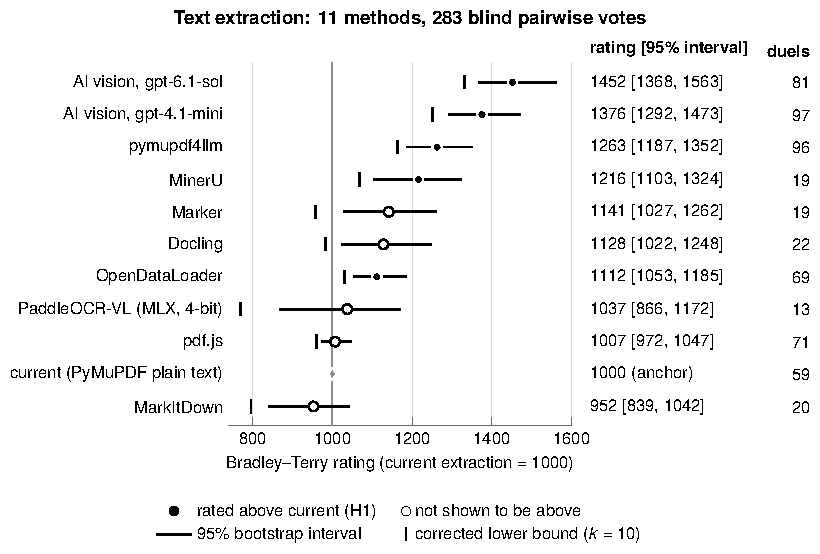
\includegraphics[width=\textwidth,height=0.85\textheight,keepaspectratio]{f20-parser-benchmark}
  \caption{Text extraction benchmark: Bradley--Terry ratings of eleven methods from 283
   blind pairwise votes over 24 pages, pooled over four comparisons and
   anchored at the current production extraction (1000). Filled dots mark the
   five methods whose Bonferroni-corrected lower bound ($k=10$) lies above 1000,
   which is the test of hypothesis H1.}
  \label{fig:parser-bench}
\end{figure}

\paragraph{Result.} \Cref{fig:parser-bench} shows the pooled ratings. The two
vision models lead, with 1452 and 1376 points, followed by pymupdf4llm at 1263
and MinerU at 1216. The other six challengers lie between 952 and 1141, and
current sits at its anchor of 1000. H1 holds: five methods pass, the two
vision models, pymupdf4llm, MinerU, and OpenDataLoader. Marker and Docling
score more points than OpenDataLoader but do not pass: with only 19 and 22
duels, their lower bounds stay below 1000.

The result needs three qualifications. First, OpenDataLoader's pass does not
hold up. It fails on the 133 first-round votes alone, and it fails again when
the bootstrap resamples whole pages instead of single votes, which respects
that the votes on one page are not independent. The other four pass both
checks, which we added after the result, in November
(\code{docs/\allowbreak thesis/\allowbreak experiments/\allowbreak parser-benchmark/\allowbreak analysis/}).
Second, the intervals of the two vision models overlap, so their order is
unsettled. Third, in the first comparison ``both unusable'' was the most
frequent answer for the current extraction, in 31 of its 39 duels. These
verdicts were quick, 22 of the 31 under five seconds, and fell late in one
sitting of 108 duels, so they record that the text looks unusable at a glance,
not a reading of both outputs.

\paragraph{Where the methods differ.} Automatic checks over the same 24 pages
show that the current extraction carries the running footer into the content
on 23 of them. The methods that strip the footer, OpenDataLoader, Marker, and
MinerU, do not lead, while the two vision models copy it on 8 and 18 pages,
because their prompt asks for everything that the page prints; so the footer
explains only part of the ranking. pymupdf4llm runs
its own OCR pass, optical character recognition on the page image, on pages it
judges image-heavy, which is part of why it scores well and which production
would have to switch off.

\paragraph{Cost.} Measured on an 8\,GB Mac, the current extraction takes at
most 0.06 seconds per page at about 62\,MB of memory, and pymupdf4llm, with its
OCR pass on, under a second at about 390\,MB
(\code{docs/\allowbreak thesis/\allowbreak experiments/\allowbreak parser-benchmark/\allowbreak PROTOCOL.md}).
The heavy engines take 1.2 to 5.8 seconds per page and 0.9 to 3\,GB of memory,
not counting what they allocate on the GPU, and each needs a model download of
0.5 to 1.7\,GB. On the 4\,GB production machine, which also runs the API, the
worker, and two Redis instances, they are not an option. The two vision models
together cost \$0.21 for the 24 pages at list prices, under a cent per page,
at 1.8 to 5.7 seconds per page, and the page leaves the server; the fee is
paid per page and per uploader. Production's OpenAI vision calls use neither
model: they run on the code default \code{gpt-4o-mini}, because the model
variables were never set. The benchmark therefore describes the vision path
with \code{gpt-4.1-mini} set, not the path as deployed.

\paragraph{Threats.} We named these in the protocol before the result. The
judge is the author of the product. The automatic checks use PyMuPDF's own
text layer as reference, which favours two of the methods. The 24 pages come
from one university and hold no scan, duels within a comparison are not
independent, later comparisons were less blind, and the heavy engines saw a
60-page excerpt.
We corrected for none of this. Two further threats are not in the protocol.
First, methods that emit headings, lists, and tables gain typography in the
benchmark's viewer that plain text does not, so the benchmark measures which
rendered output a reader prefers. Second, the real consumers of the text are
models, for synthesis, quiz, and retrieval, and we did not measure whether the
preference carries over to them; a retrieval run per extractor would test it.
No second rater judged any subset either, so how far the result depends on the
one judge is unknown.

\section{Answer to RQ1}
\label{sec:c4-answer}

Our answer to the first part of RQ1 has three steps. The learner who uploads
a PDF reads it at once, while the worker writes each generated page as soon as
it exists. Before any model call, a deterministic plan finds the boilerplate,
gives each page a role, and picks the pages that the title and quiz steps
read. Then one rule decides from the page itself whether a text model or a
vision model reads it. On 1{,}593 pages of real decks, the old rule sent to
vision only 12 pages without teaching text and no page with a figure, the new
rule 87, among them 52 of the 53 pages that the author labelled as needing
their image; as these pages were the rule's calibration set, the 52 are a fit,
not an accuracy.

For the second part, the author, judging blind under a pre-registered
protocol, preferred the transcription of the stronger vision model to the
current extraction at more than 10:1 in expected score, and that of the
smaller one at about 9:1, each for under a cent a page. pymupdf4llm followed
at about 4.5:1, without a fee and, on an 8\,GB Mac, at under a second more per
page with its OCR pass on. The heavy layout engines need 0.9 to 3\,GB of
memory, which the 4\,GB production machine cannot spare beside the API, the
worker, and two Redis instances. We did not change the production extractor on
this basis at the pin.

One judge chose between rendered outputs of 24 born-digital pages from one
university, and we did not test whether the models that read the text do
better with the preferred version. Nor did we measure how soon a generated
page arrives, what a deck costs, whether the generated text is grounded in its
page, or whether any of this helps learning. The reliability of the pipeline
rests on its design, on tests of each mechanism, and on 115 production parses
under light load, 16 of which failed visibly; we ran no load test, and fault
injection covers only the provider layer
(\code{tests/\allowbreak unit/\allowbreak test\_chaos\_*.py}).
\Cref{sec:future-work} proposes a combination of the two results, which we did
not test.
